\documentclass[12pt]{beamer}
\usepackage{graphicx}
\usepackage{tikz}
\usetikzlibrary{automata}


\title{PRESENTATION ON GRAPH AND DIGRAPH}

\institute{Central Department of Mathematics, Tribhuvan University\\Kirtipur,  Kathmandu, Nepal}
\date{\today}
\begin{document}
\begin{frame}


\maketitle
\end{frame}
\section{ Isomorphism}
\begin{frame}{Isomorphism}
        
	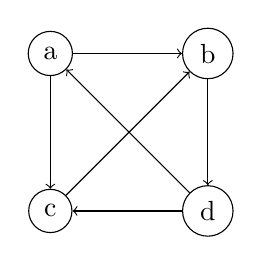
\begin{tikzpicture}
	\node[circle ,draw=black](v1)at(0,0){a};
	\node[circle,draw=black](v2) at (2,0){b};
	\node[circle,draw = black](v3) at(0,-2) {c};
	\node[circle,draw = black](v4) at(2,-2){d};
	\draw[->](v1)--(v2);
	\draw[<-](v2)--(v3);
	\draw[<-](v3)--(v4);
	\draw[->](v4)--(v1);
	\draw[->](v1)--(v3);
	\draw[->](v2)--(v4);
	\end{tikzpicture}
	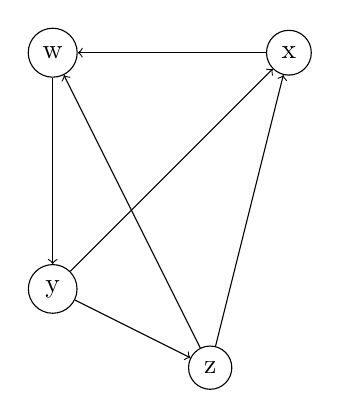
\begin{tikzpicture}
	\node[circle ,draw=black](v1)at(0,0){w};
	\node[circle,draw=black](v2) at (3,0){x};
	\node[circle,draw = black](v3) at(0,-3) {y};
	\node[circle,draw = black](v4) at(2,-4){z};
	\draw[<-](v1)--(v2);
	\draw[<-](v2)--(v3);
	\draw[->](v3)--(v4);
	\draw[->](v4)--(v1);
	\draw[->](v1)--(v3);
	\draw[<-](v2)--(v4);
	\end{tikzpicture}
	\end{frame}
	\begin{frame}{Cartesian Product}
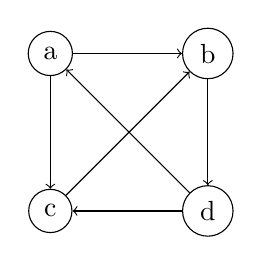
\begin{tikzpicture}
\node[circle ,draw=black](v1)at(0,0){a};
\node[circle,draw=black](v2) at (2,0){b};
\node[circle,draw = black](v3) at(0,-2) {c};
\node[circle,draw = black](v4) at(2,-2){d};
\draw[->](v1)--(v2);
\draw[<-](v2)--(v3);
\draw[<-](v3)--(v4);
\draw[->](v4)--(v1);
\draw[->](v1)--(v3);
\draw[->](v2)--(v4);
\end{tikzpicture}
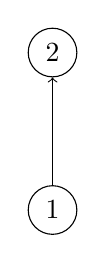
\begin{tikzpicture}
\node[circle ,draw=black](v1)at(2,2){2};
\node[circle,draw=black](v2) at (2,0){1};
\draw[->](v2)--(v1);
\end{tikzpicture}
\end{frame}
\begin{frame}
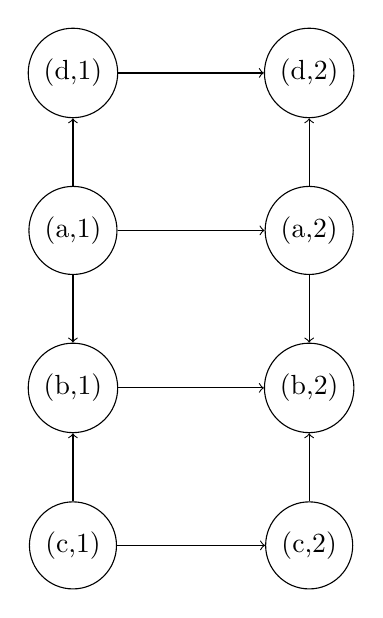
\begin{tikzpicture}
\node[circle ,draw=black](v1)at(0,0){(a,1)};
\node[circle,draw=black](v2) at (3,0){(a,2)};
\node[circle,draw = black](v3) at(0,-2) {(b,1)};
\node[circle,draw = black](v4) at(3,-2){(b,2)};
\node[circle,draw=black] (v5) at (0,-4){(c,1)};
\node[circle, draw= black] (v6) at (3,-4) {(c,2)};
\node[circle, draw = black] (v7) at (0,2) {(d,1)};
\node[circle, draw = black] (v8) at (3,2) {(d,2)};
\draw[->](v1)--(v2);
\draw[->](v1)--(v3);
\draw[->](v3)--(v4);
\draw[->](v2)--(v4);
\draw[->](v5)--(v6);
\draw[->](v5)--(v3);
\draw[->](v6)--(v4);
\draw[->](v7)--(v8);
\draw[->](v1)--(v7);
\draw[->](v2)--(v8);
\end{tikzpicture} \\

\end {frame}




\end{document}
